\documentclass{article}[12pt]

% Math & clever spacing
\usepackage{amsmath}
\usepackage{amssymb}
\usepackage{xspace}

% Graphics and colors
\usepackage{graphicx}
\usepackage{xcolor}
\usepackage{color}

% disable subsubsections in the TOC
%\makeatletter
%\def\l@subsubsection#1#2{}
%\makeatother

% Fix the appendix lines in the TOC
%\renewcommand*{\appendixname}{}

% Line number every fifth line
%\modulolinenumbers[5]
%\linenumbers

\usepackage[top=1in, bottom=1.25in, left=0.75in, right=0.75in]{geometry}

\usepackage[T1]{fontenc}
\renewcommand*\rmdefault{ptm}

\usepackage{hyperref}
\usepackage{listings}
\usepackage{url}
\usepackage{tablefootnote}
\usepackage{fancyhdr}
\usepackage{lastpage}
\usepackage{longtable}
\pagestyle{fancy}

\fancyhead{}
\fancyfoot{}
\fancyhead[LO,LE]{LCA-13501}
\fancyhead[CO,CE]{FITS Format Specification for Science Rafts}
\fancyhead[RO,RE]{Page \thepage~of \pageref{LastPage}}  %\pageref{lastpage}}

\usepackage{alltt}

% Title page 
\title{Specification for FITS Image Files from Raft and Focal Plane-Level Electro-Optical Tests}

\newcommand{\red}{\textcolor{red}}
\newcommand{\blue}{\textcolor{blue}}
\definecolor{darkgreen}{rgb}{0.0, 0.7, 0.0}
\newcommand{\green}{\textcolor{darkgreen}}

\allowdisplaybreaks

% Body of the document
\begin{document}

\maketitle
\tableofcontents
\newpage
\listoftables

\section{Change History}
Initial draft in progress.  \red{Issues for discussion are highlighted in red.}\

\red{3 June:  Some clarifications in tables, clean-up of text}

\red{1 June:  Corrected description of the origin of the Raft coordinate system.}

\red{1 June:  Switched from CD to PC/CDELT keywords for representing the WCS coordinates} 

\red{31 May:  Corrected WCS CRVAL2 specifications for horizontal pre-scan.}

\red{20 May:  Added DTM/DTV keyword specifications to define the pixel coordinates for an assembled single-CCD image}

\red{19 May:  Added Mosaic DETSIZE, DATASEC, and DETSEC specifications for single-sensor image assembly with trimming.  The WCS CD keywords may change to PC/CDELT; this would be a minor change not affecting any of the calculations.}

The source for this draft, including ASCII versions of the example headers, is maintained at \url{https://github.com/lsst-camera-dh/RaftFitsSpec}.

\section{Scope}
This document describes the naming, organization, and formats of the FITS files from Science Raft-level and focal plane-level (i.e., more than one raft) electro-optical tests.  The definitions of other data products related to raft and focal plane-level metrology will be described elsewhere.

\section{Acronyms}

\section{References}

[1] LCA-10140 Specification for FITS Images from Electro-Optical Tests

\noindent{[2] LSST-1614 LSST Camera Coordinate and Numbering Systems}

\noindent{[3] LSST-13381 LSST Camera Detector Plane Layout}

\noindent{[4] Definition of the Flexible Image Transport System (FITS), v3.0, \url{http://fits.gsfc.nasa.gov/standard30/fits_standard30aa.pdf}}

\noindent{FITS references and resources are collected here:  \url{http://fits.gsfc.nasa.gov}.}

\section{Introduction}
This document extends the definition of formats and naming conventions for single-sensor image files [1] to images taken at the raft level (i.e., nine sensors), or collections of rafts up to the entire focal plane.  As for single sensors, the image files will be in FlTS format, long in widespread use in astronomy.  The FITS standard is well defined and many i/o libraries and tools exist to read, write, manipulate, and display data stored in FITS format.  The format consists of keyword-value pairs in ASCII headers together with (typically) binary image data or tables.  A header and associated data are together called a Header Data Unit, and a FITS file can contain any number of these.

Raft-level images will be generated with Test Stand 8 (TS8).  Focal plane-level images will be generated with the Bench for Optical Testing (BOT).  BNL and SLAC will each have a TS8.  The BOT will be at SLAC.  The specifications in this document are to ensure portability of the image data products across sites, to provide a well-defined common interface for the analysis scripts, to define pixel coordinate keywords for image assembly by display tools (specifically ds9 and Firefly), and to facilitate curation of raft and camera test data.

As for sensor acceptance testing, raft and focal plane-level image files will be used for any of a variety of analyses, depending on the set-up of the test stands, including Flat Field Exposures, Pocket-Pumping Exposures, Dark Integrations, Fe-55 X-ray Exposures, Wavelength Scan, Superflat Images, Spot Imaging Exposures, Readout System Noise Images, and Readout System Crosstalk Images.
The format specifications of the image files from these tests are very similar but some tests have test-specific keywords.  

The specifications of the file and directory naming conventions, and of the FITS headers derive from the corresponding specifications in LCA-10103 for single sensor testing.

\section{File Naming and Directory Structure}
Considerations of human readability, data curation, and automated processing motivate specification of conventions for naming and organization of the image files.

\subsection{Directory Structure}

The directory structure for raft-level measurements is designed to extend from measurements with single rafts (in TS8) to entire focal planes (with the BOT).  The naming convention is:

\red{{\bf rafts/<institution>/sraft<raft number>/<acquisition type>/<job ID>/s<CCD number>} }

%\red{N.B. This organization is not currently possible with the Job Harness system}

%\red{TBD: expand <test type> to list the acquisition and analysis directories actually used?  Possibly limit to just the acquisition directories - this document is not defining specs for the analysis results directory/file naming or formats}
%\red{Are there other acquisition types to be listed?  The directories with analysis results, and the results files themselves provisionally are not included in this specification.}

%\red{Subdirectories for sensor names/raft locations}

\begin{table}
\begin{centering}
\begin{tabular}{| l | l |}
\hline
{\bf Quantity} & {\bf Description} \\
\hline
%{\bf rafts} & A designator to distinguish from {\bf CCDs} for single-sensor data sets \\
{\bf <institution>} & {\bf bnl} or {\bf slac} \\
{\bf sraft<\#\#>} & Designator of the science raft (each \# = 0--4) \\
{\bf <acquisition type>} & {\bf dark\_acq, fe55\_acq, flat\_acq, lambda\_acq, ppump\_acq, qe\_acq, read\_noise, spot\_acq} \\
{\bf <job ID>} & Job ID number assigned by the Job Harness \\
{\bf <s\#\#>} & Location designator of the sensor in the raft (each \# = 0--2) \\
\hline
\end{tabular}
\caption{Definitions of the components of the directory names for image data./label{tab:dir}}
\end{centering}
\end{table}

%{\bf Use the same designators for test type as in the EO test directories?}

%\red{These directories may contain subdirectories, perhaps depending on the test type...}


\subsection{File Names}

The file names for a given sensor, test type, and processing step shall be of the form

%<sensor id>_<test type>_<image type>_<seq. info>_<time stamp>.fits
{\bf <CCD id>\_<test type>\_<image type>\_<seq. info>\_<time stamp>.fits }


\red{TBD:  Include metrology files}

\begin{table}
\begin{centering}
\begin{tabular}{| l | l |}
\hline
{\bf Quantity} & {\bf Description} \\
\hline
%{\bf <CCD id>} & {\bf s{\tt \#\#}}, where {\tt \#\#} are the coordinates of the CCD in the raft; each \# = 0--2, as defined in [2] \\
{\bf <CCD id> } & {\bf LSST Serial Number, e.g. E2V-CCD250-\#\#\# or ITL-3800C-\#\#\#} \\
{\bf <test type>} & {\bf dark, fe55, flat, lambda, spot} \\
{\bf <image type>} & One of bias, dark, fe55, or flat \\
{\bf <seq. info>} & Normally a 3-digit sequence number such as 000, 001, 002. \tablefootnote{Photon Transfer Curve data (pairs of flats) shall have exposure times and flat1/flat2 designators, e.g., 0010.0s\_flat1} \\
{\bf <time stamp>} & A string of the form YYYYMMDDHHMMSS recording UTC of the start of the image acquisition\\
\hline
\end{tabular}
\caption{Definitions of the components of the file names for image data.\label{tab:file}}
\end{centering}
\end{table}

\red{An example with the desired directory path:}

\red{{\tt rafts/bnl/sraft22/dark\_acq/361/s12/E2V-CCD250-088\_dark\_dark\_003\_20160121191343.fits}}


\section{Internal File Organization}

The image files are multiple-extension FITS files with basic (not site-specific) information in the primary header, then 16 image extensions (one per segment), followed by test condition, CCD operating condition, and site-specific extension(s).  For the latter, examples are given here but are not formally part of the specification.  

{\bf N.B.:} The analysis scripts should not depend on information in the site-specific extensions.

\subsection{Image Extensions}

The naming of the segments is defined in [2].  Each segment has a 2-digit designator, and these are incorporated in the {\tt EXTNAME} keyword strings as indicated in the example header below.

The headers of the image extensions also define the pixel coordinate systems for the segments, sensors, and rafts.  These use a combination of NOAO Mosaic keyword conventions as in [1] and FITS World Coordinate System (WCS) definitions (ref).  The definitions specify which regions of the segments are pre-scan and over-scan regions.  (For TS8 a focal-plane level definition of the pixel coordinates is not needed.)

\section{Example Headers}

\subsection{Primary Header}
This example is the primary header of an image file for an ITL sensor, although the primary header is not sensor-specific.  It goes without saying that values of many of the keywords in actual data files will be different.  Keyword values are shown here and in the other example headers as a guide to the format.

%\red{
%Points for discussion:
%\begin{itemize}
%\item{LSST\_NUM, defined as the LSST-assigned serial number, is in LCA-10140 but not here}
%\item{MONOCH-SLIT\_C, AMP0-AZERO, and AMP2-ZERO\_CHECK keywords below are not in LCA-10140.}
%\item{Are the BINX and BINY keywords useful?}
%\item{LCA-10140 has DATE/MJD as the creation date of the file.  These is not in the example header below.}
%\item{MJD-OBS, the MJD date of the image acquisition, is not in LCA-10140}
%\item{What are the possible values of IMGTYPE?}
%\end{itemize}
%}

\begin{table}
\begin{alltt}
\input{primary_header.txt}
\end{alltt}
\caption{Example primary header.\label{tab:primary}}
\end{table}

\subsection{Image Extension Header (ITL)}
This example is the first image extension of an image file for an ITL sensor.  The other 15 extensions are of course similar but differ in the keywords specifying the mapping of amplifier (segment) coordinates to coordinates within a sensor, raft, or focal plane.  The calculation of these keyword values is provided in \S~\ref{sec:pixelcoords}.
%\ref{sec:coords_itl}.

\begin{table}
\tiny
\begin{alltt}
\input{image_header_seg10_ITL.txt}
\end{alltt}
\caption{Example header of an image extension for an ITL sensor. \label{tab:image_ITL}}
\end{table}

\subsection{Image Extension Header (e2V)}

This is an example of an image extension for an e2V sensor.  It is the first segment (Segment10) in the file.

\begin{table}
\tiny
\begin{alltt}
\input{image_header_seg10_E2V.txt}
\end{alltt}
\caption{Example header of an image extension for an e2V sensor.\label{tab:image_e2V}}
\end{table}

\subsection{Test Conditions Header}

\red{
\begin{itemize}
\item{Will REB-related keywords be in this extension or in an extension of their own?}
\item{What are the allowed values of the FILTER keyword?}
\item{LCA-10140 has the MONOWL keyword (Monochromator wavelength setting), but it is not in the example header}
\item{LCA-10140 has PD\_SER (Monitor Photodiode serial number), but this keyword is not in the example header.}
\end{itemize}
}

\subsection{Photodiode Readings Header}

\red{
\begin{itemize}
\item{This is a placeholder for photodiode current readings.  This may be a FITS binary table.  It probably needs to be the last extension in the file.}
\end{itemize}
}

\begin{table}
\begin{alltt}
\input{test_cond_header.txt}
\end{alltt}
\caption{Example Test Conditions extension header.\label{table:test_cond}}
\end{table}

\subsection{CCD Conditions Header}

\red{
\begin{itemize}
\item{The CCD\_COND headers are just placeholders in recent single sensor image files.  Are they needed?  In LCA-10140 they contained keywords defining currents and voltages for the segments.  These probably were controller settings rather than read-out values.}
\end{itemize}
}

\begin{table}
\begin{alltt}
\input{ccd_cond_header.txt}
\end{alltt}
\caption{Example CCD Conditions extension header.\label{table:ccd_cond}}
\end{table}


\section{Pixel Coordinate Mapping\label{sec:pixelcoords}}
This section describes the calculations for mapping segments to sensors, rafts, and the focal plane, defining the shifts and rotations to make continuous pixel coordinate systems.  The pixel coordinate systems are based on the nominal layout of the rafts and focal plane as defined in [3], and are intended to be used primarily for visualization during I\&T of Science Rafts and of the Camera focal plane.  The relevant diagrams of [3] are reproduced in Figures 1--3.  The segments, CCDs, and rafts each have two-digit identifiers that correspond to their x, y locations in the layout.

The transformations are developed here in terms of the FITS World Coordinate System (WCS) keyword specifications for FITS image data [ref].  The next subsection describes the WCS FITS keywords used.

%That is, describe how to derive the values for the MOSAIC and WCS keywords.

%The focal plane layout defined in [3] specifies the nominal locations of the rafts and the sensors within the rafts.


\subsection{Important Conventions}
Note that the layout is represented in [3] as viewed through L3, i.e., looking down on the CCDs.  In this orientation, the x direction of the Camera Coordinate System is toward the $left$ and the y direction is $up$.  This convention is adopted here.  Note also that by this convention, the nominal x (serial) direction of a sensor is oriented along the y direction of the Camera Coordinate System.  

By convention for FITS image data, the first pixel in an image has coordinates (1, 1).  This is adopted here for sensors and rafts.  In particular, the first pixel in an assembled raft image is assigned to the lower right corner of the raft.  This pixel is not within a CCD (see Fig. 2). 

For focal plane-level images, the origin of the pixel coordinate system is defined as if a Raft 00 were present.  That is, pixel (1, 1) would have been in segment 00 of CCD 00 in Raft 00.  The only other potential reference point, the center of the Camera focal plane (i.e., the center of CCD 11 in Raft 22) has the disadvantage of being between pixels, and adopting it as the origin would mean including 0.5 pixel offsets for pixel coordinates measured with respect to it.

\subsection{Pixel Coordinate Transformations}
In the following $S$ is the segment location designator (00, 01...07, 10, 11, ...17) in a CCD, $C$ is the CCD location designator in a raft (00, 01, 02, 10, 11, 12, 20, 21, 22), and $R$ is the raft location designator in the focal plane (see Fig. 3).  Where useful, these designators are decomposed into their x and y index values, e.g., $S = 10 \times S_x + S_y$.  Keep in mind that x and y index values increase along the x and y directions, respectively, in the Camera coordinate system.

Also defined below are s (serial) and p (parallel) coordinates, which are useful for assembling single CCD and raft-level images oriented with the {\bf serial direction horizontal}.  (The NOAO Mosaic keywords, also defined below, assemble segment images this way for single CCDs.  The value of the s and p coordinates primarily will be for raft-level images.)  Where convenient the $S$ designator will be decomposed into s and p index values, e.g., $S = 10 \times S_p + S_s$.

\begin{figure}
\centering
    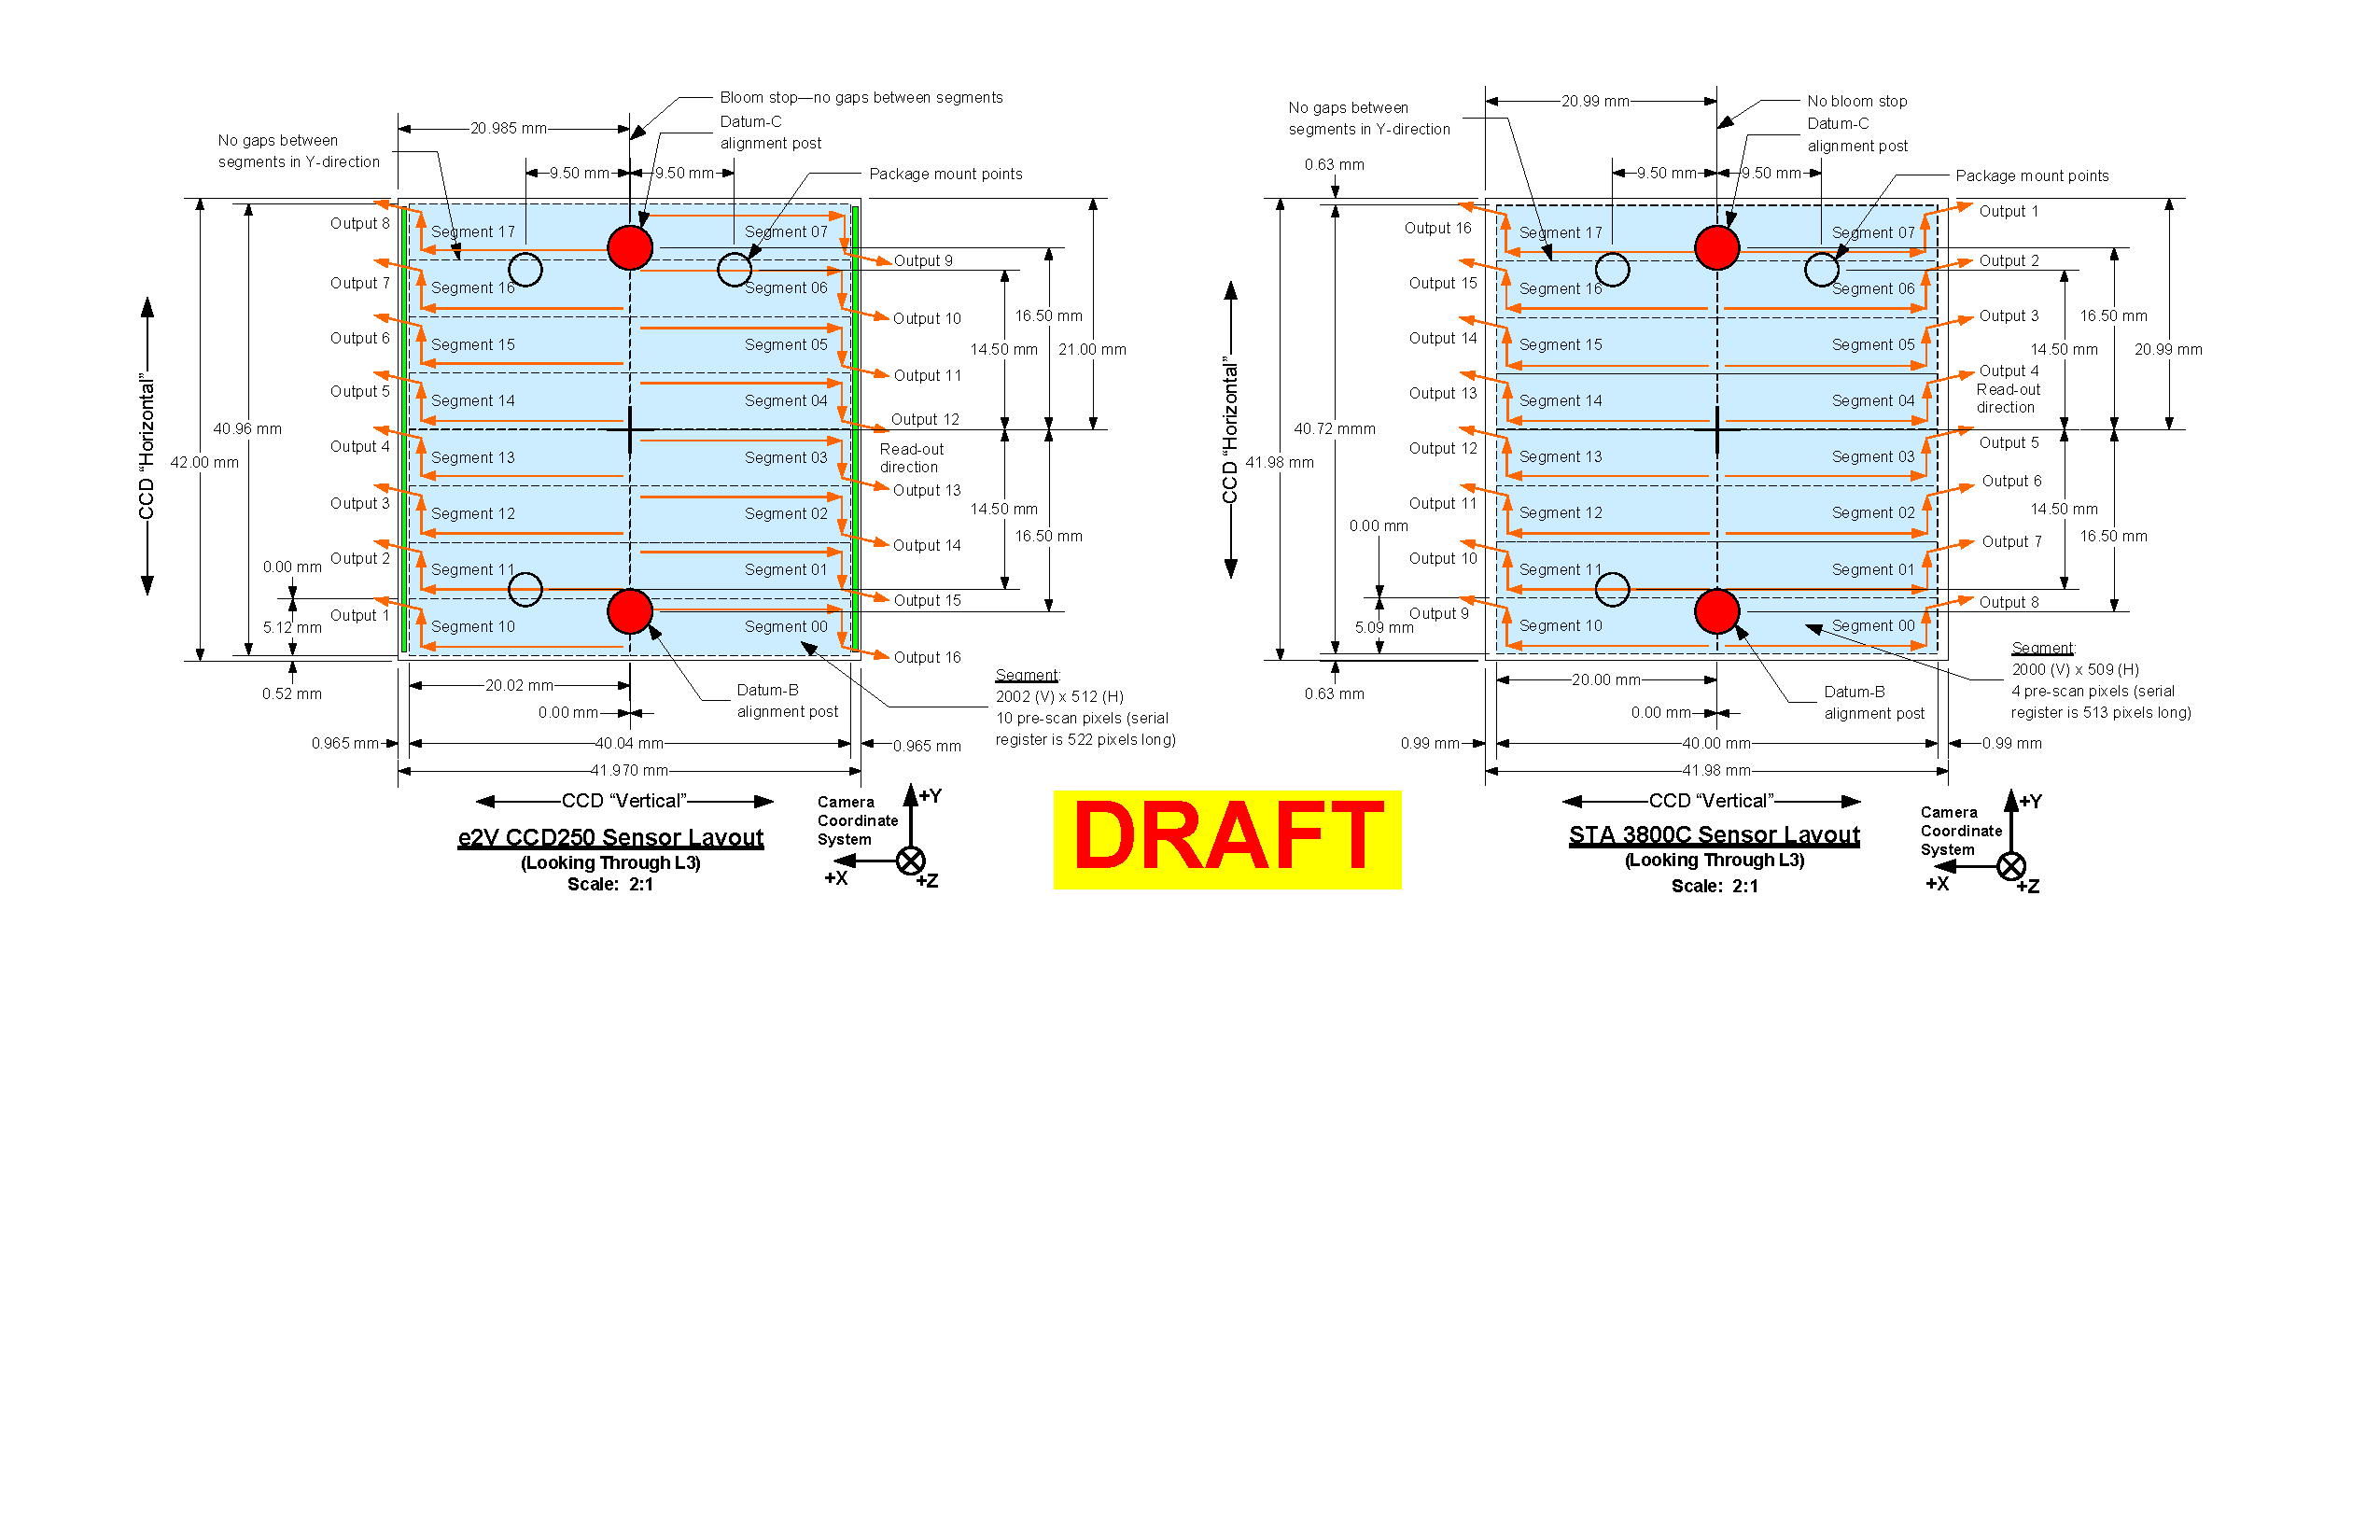
\includegraphics[width=0.95\textwidth]{sensor_layout.pdf}
    \caption{Dimensions and segment layouts for e2V {\it (left)} and ITL {\it (right)} CCDs.  Note that the camera coordinate system has the x axis oriented along what is the $-$y direction for single-sensor assembled images.  These images are from [3].}
    \label{fig:sensor}
\end{figure}

\begin{figure}
\centering
    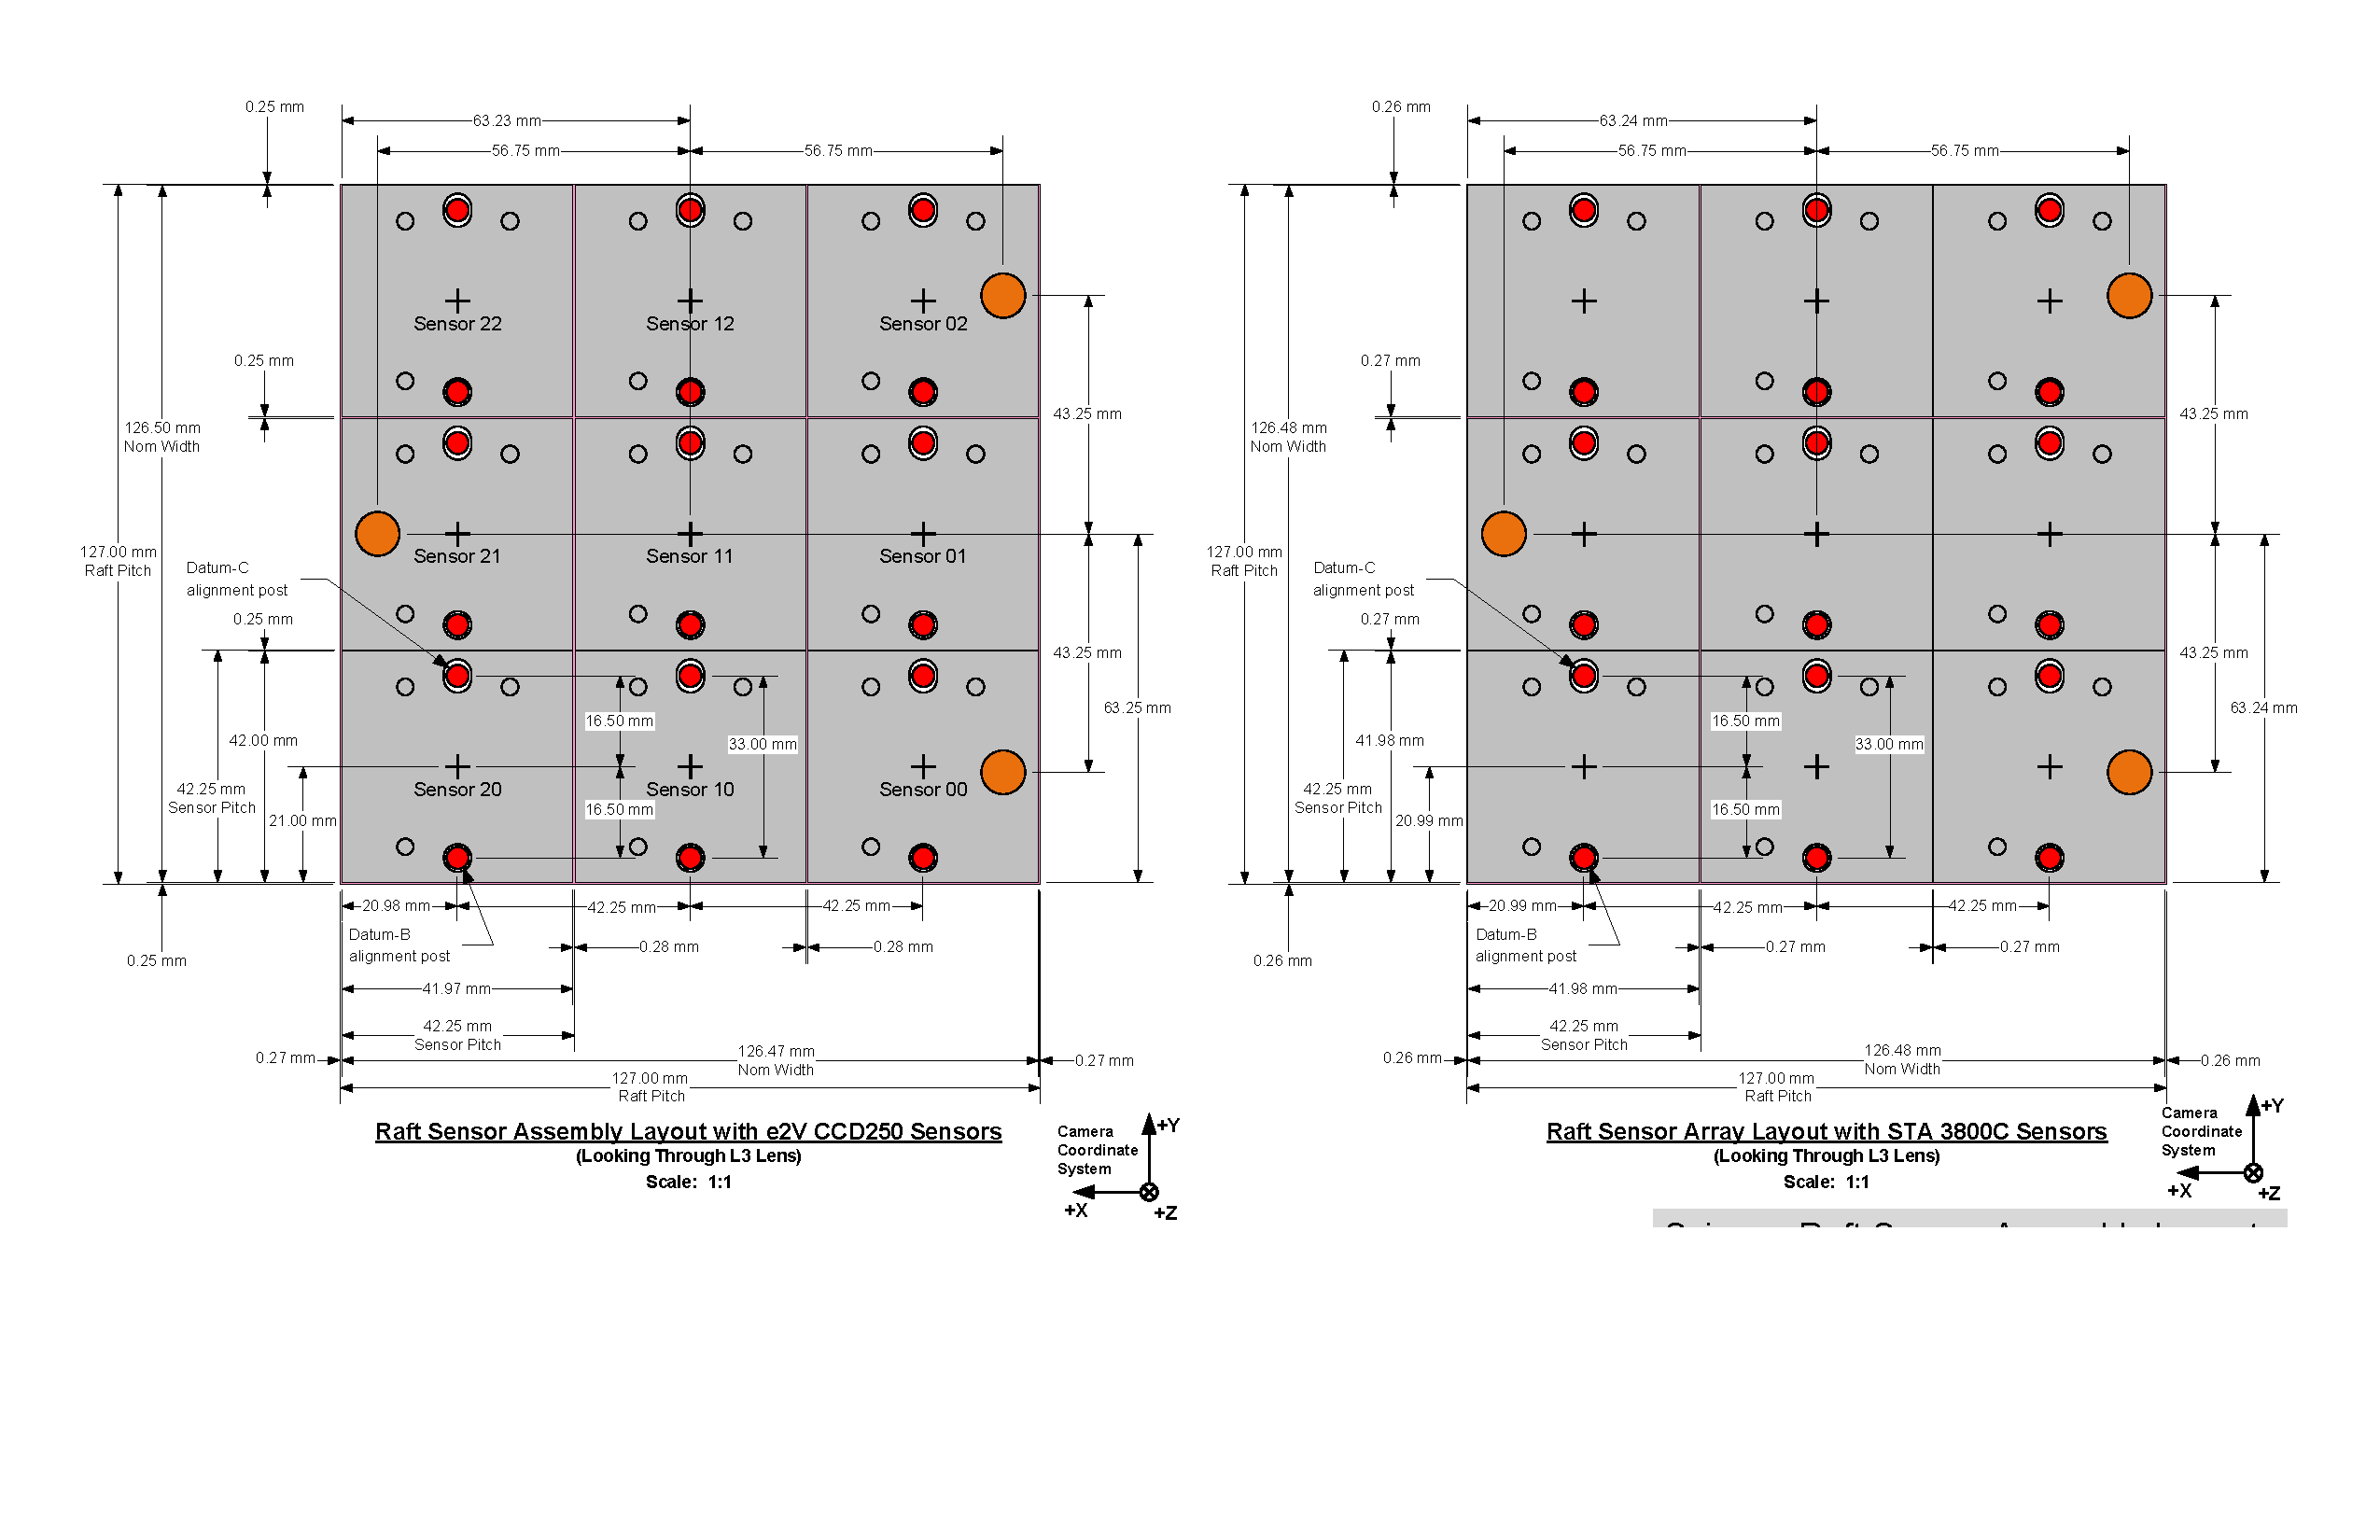
\includegraphics[width=0.95\textwidth]{raft_layout.pdf}
    \caption{Dimensions and sensor layouts for e2V {\it (left)} and ITL {\it (right)} Science Rafts.  These images are from [3].}
    \label{fig:raft}
\end{figure}

\begin{figure}
\centering
    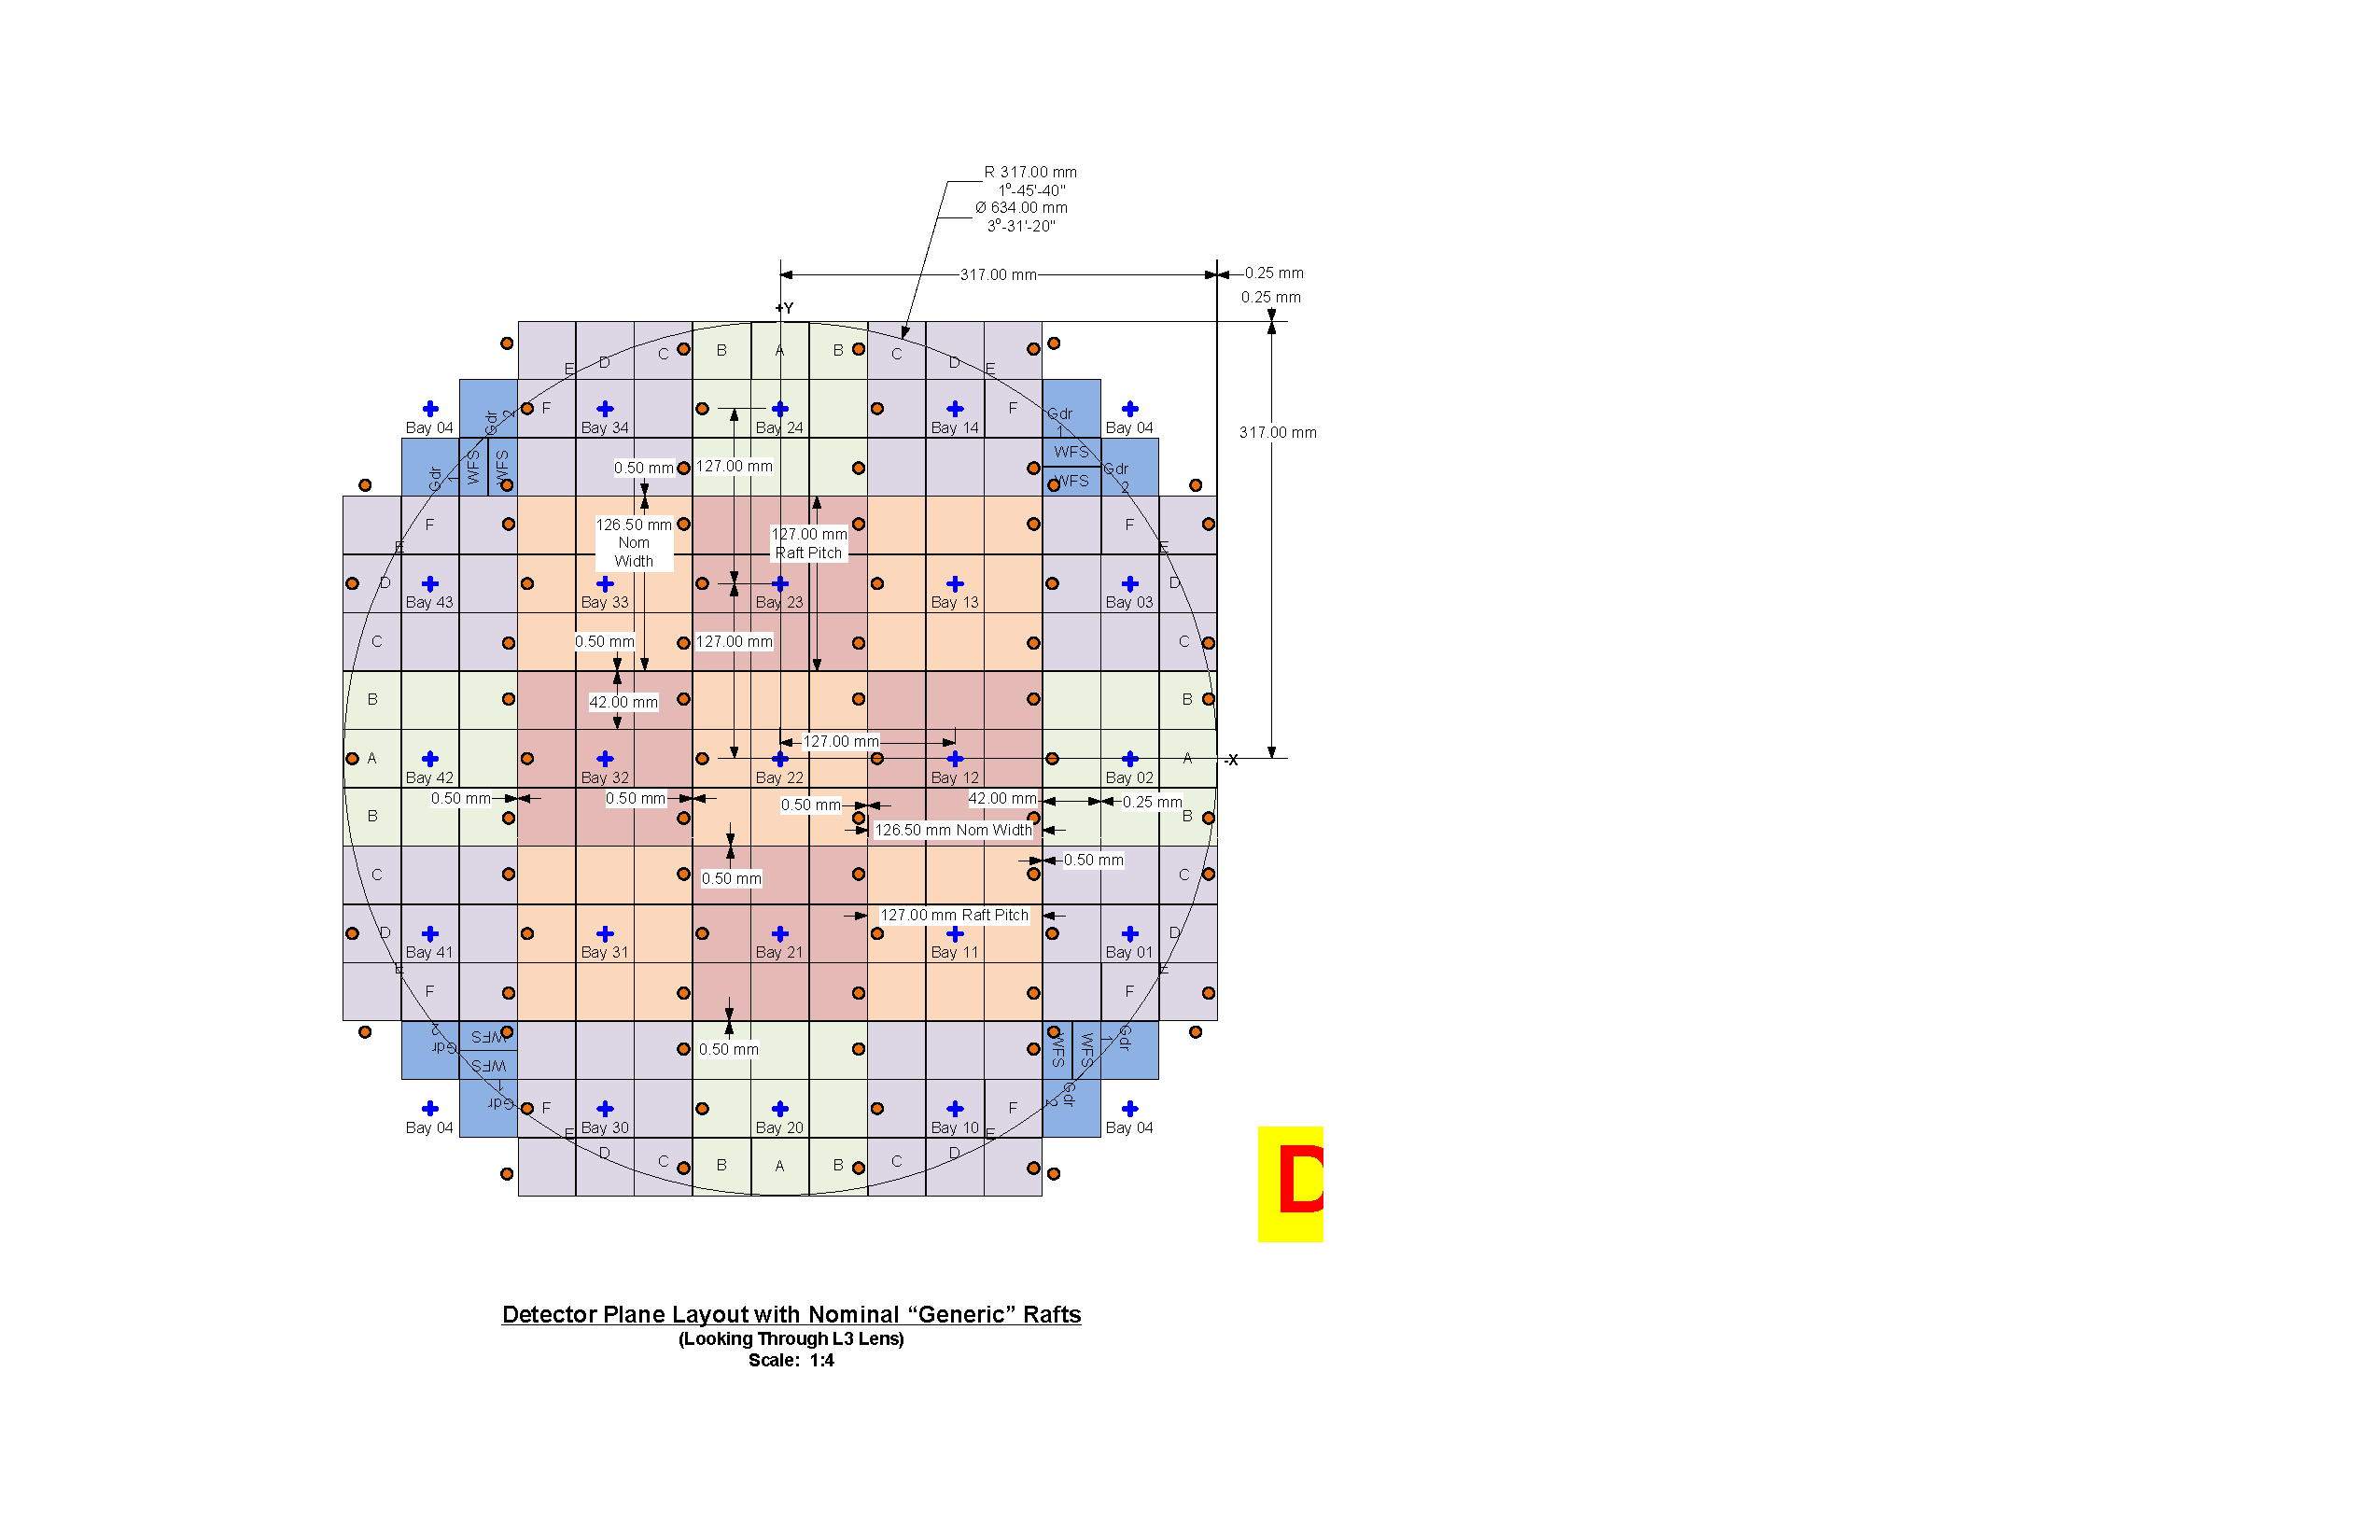
\includegraphics[width=0.75\textwidth]{focal_plane_layout.pdf}
    \caption{Dimensions and arrangements of the rafts in the focal plane, from [3].}
    \label{fig:focalplane}
\end{figure}

\subsection{Dimensions and Pitch}
The relevant quantities for defining the pixel coordinate systems are listed in Table~\ref{tab:dims}.  All are extracted from the diagrams in [3].  The column {\bf Designator} lists the name of the corresponding variable in the algorithmic description of the coordinate calculation.  

{\bf N.B.:} These variables are defined in terms of equivalent pixels, i.e., they are the physical dimensions divided by the pixel size.

\begin{table}
\begin{centering}
\begin{tabular}{| l | c | c | c |}
\hline
{\bf Quantity} & {\bf e2V CCD} & {\bf ITL CCD} & {\bf Designator} \\
\hline
%Pixel size & 10~$\mu$m $\times$ 10~$\mu$m & 10~$\mu$m $\times$ 10~$\mu$m & -- \\
Segment pixels & $2002 \times 512$ (vertical $\times$ horizontal) & $2000 \times 509$ & dimv $\times$ dimh \\
Active area  (x $\times$ y) \tablefootnote{Note that the dimensions are specified here in terms of the orientation of the CCDs in the raft.} & 4004  $\times$ 4096 & 4000 $\times$ 4072  & ccdax $\times$ ccday \\
CCD physical size & 4197 $\times$ 4200 & 4198 $\times$ 4198 & ccdpx $\times $ ccdpy \\
%Pitch of CCDs & 4225 $\times$ 4225 & 4225 $\times$ 4225 & -- \\
Inter-CCD gaps & 28 $\times$ 25 & 27 $\times$ 27 & gap\_inx $\times$ gap\_iny \\
Pitch of rafts & 12700 $\times$ 12700 & 12700 $\times$ 12700 & raftx $\times$ rafty \\
Gaps at edges of rafts & 26.5 $\times$ 25 & 26 $\times$ 26 & gap\_outx $\times$ gap\_outy \\
\hline
\end{tabular}
\caption{CCD and raft-related dimensional quantities for the pixel coordinate systems, from [3].  The physical dimensions have been converted to pixels for the nominal 10~$\mu$m $\times$ 10~$\mu$m pixel size.\label{tab:dims}}
\end{centering}
\end{table}


%\begin{table}
%\begin{tabular}{| l | c | c | c |}
%\hline
%{\bf Quantity} & {\bf e2V Raft} & {\bf ITL Raft} & {\bf Designator} \\
%\hline
%Pitch of CCDs & 4225 $\times$ 4225 & 4225 $\times$ 4225 & -- \\
%Inter-CCD gaps & 28 $\times$ 25 & 27 $\times$ 27 & gap\_inx $\times$ gap\_iny \\
%Pitch of rafts & 12700 & 12700 & raftx $\times$ rafty \\
%Gap at edges of rafts & 27 $\times$ 25 & 26 $\times$ 26 & gap\_outx $\times$ gap\_outy \\
%\hline
%\end{tabular}
%\caption{Science Raft-related dimensional quantities for the pixel coordinate systems.  The physical dimensions have been converted to pixels for the nominal 10~$\mu$m $\times$ 10~$\mu$m pixel size.\label{tab:raft}}
%\end{table}

%\red{CCS does not transpose or invert any of the individual segment images, right?}

Let $(x_s, y_s)$ denote pixel coordinates in a given segment $S$, as read out, so that $x_s$ is in the serial direction and $y_s$ is in the parallel direction, and consider them to be in as-read-out order, without transpositions to account for the locations of the output nodes.  If $S$ is in CCD $C$ and the CCD is in raft $R$, then the pixel coordinates in each system can be defined as follows.

Keeping in mind that the CCD is oriented as in Figure 1 (i.e., rotated so the parallel direction is horizontal), then the corresponding pixel coordinates in the CCD system are 
\begin{equation}
x_c = y_s (1 - S_x) + (2 \times {\rm dimv} + 1 - y_s)  S_x
\end{equation}

and (for e2V CCDs)

\begin{equation}
y_c = (x_s + S_y \times {\rm dimh})  (1 - S_x) + [1 - x_s + (S_y + 1) \times {\rm dimh}] S_x
\end {equation}
or (for ITL CCDs)

\begin{equation}
%y_c = (1 - x_s + (S_y  + 1) \times {\rm dimh} )  (1 - S_x) + [1 - x_s + (S_y + 1) \times {\rm dimh}] S_x
y_c = 1 - x_s + (S_y  + 1) \times {\rm dimh} 
\end{equation}

The corresponding pixel coordinates in the raft are:

\begin{equation}
x_r = x_c + {\rm gap\_outx} + ({\rm ccdpx} - {\rm ccdax})/2 + C_x ( 2 \times {\rm dimv} + {\rm gap\_inx} + {\rm ccdpx} - {\rm ccdax})
\end{equation}

and

\begin{equation}
y_r = y_c + {\rm gap\_outy} + ({\rm ccdpy} - {\rm ccday})/2 + C_y ( 8 \times {\rm dimh} + {\rm gap\_iny} + {\rm ccdpy} - {\rm ccday})
\end{equation}

And the corresponding coordinates in the focal plane are:

\begin{equation}
x_f = x_r + R_x \times {\rm raftx}
\end{equation}

and

\begin{equation}
y_f = y_r + R_y \times {\rm rafty}
\end{equation}

%N.B. The actual separation between the edges of adjacent rafts is twice the gap sizes listed in the last entry of the table above.

%The dimensions in the table above can be converted to equivalent numbers of pixels by dividing by 10 $\mu$m, i.e., multiplying the dimensions in mm by 100.


%The pixel coordinate system for the focal plane is approximate, of course, accounting for the nominal gaps between the sensors and rafts.  For simplicity, each raft is assigned to a fixed range of x and y pixel coordinates in the focal plane.  The differences in the pixel dimensions of E2V and ITL sensors are taken up by adjusting the gap between rafts by a small amount.  This scheme would also simplify handling a hybrid focal plane of e2V-only and ITL-only rafts.

In the serial/parallel coordinate system, which is rotated by 90$^\circ$ {\bf clockwise} from the orientation shown in Figure 2, the serial coordinate in the CCD system is (for e2V sensors)
\begin{equation}
s_c = (x_s + S_s \times {\rm dimh}) (1 - S_p) + [1 - x_s + (S_s + 1) \times {\rm dimh}] S_p
\end{equation}

and (for ITL sensors)

\begin{equation}
s_c = 1 - x_s + (S_s + 1) \times {\rm dimh}
\end{equation}

For both types of CCD the parallel coordinate

\begin{equation}
p_c = y_s  (1 - S_p) + (2 \times {\rm dimv} - y_s + 1) S_p
\end{equation}

and in the raft the serial and parallel coordinates are

\begin{equation}
s_r = s_c + {\rm gap\_outy} + ({\rm ccdpy} - {\rm ccday})/2 + C_s \times (8 \times {\rm dimh} + {\rm gap\_iny} + {\rm ccdpy} - {\rm ccday})
\end{equation}

and

\begin{equation}
p_r = p_c + {\rm gap\_outx} + ({\rm ccdpx} - {\rm ccdax})/2 + C_p \times (2 \times {\rm dimv} + {\rm gap\_inx} + {\rm ccdpx} - {\rm ccdax})
\end{equation}

{\bf N.B.:} In this serial/parallel system the serial coordinates $s_c$ and $s_r$ increase to the {\it right}.  This is {\it opposite} of what is specified in the NOAO Mosaic keywords.  At the CCD level in the serial/parallel system, Segment~00 is at the lower left.  In contrast, in the NOAO Mosaic system Segment~10 is at the lower right.  At the raft level in the serial/parallel system, Sensor~00 is at the lower left.

{\bf N.B.:} For the reason described above, the serial/parallel system, although completely and correctly defined, will not be useful for displaying coordinates on single CCD images assembled by {\it ds9}.

\subsection{World Coordinate System FITS Keywords}
The FITS World Coordinate System (WCS; see Sec. 8 of [4]) keyword specification allows multiple coordinate systems to be defined for the same image.  Each coordinate system is designated by a single letter; the letter is appended to the corresponding header keywords that define the transformation.  We take advantage of that multiple coordinate system here to define coordinate systems for individual segments ({\tt A} for Amplifier\footnote{The NOAO MOSAIC header keyword convention, which is an earlier approach to defining keywords for mapping multi-sensor images together, used the term Amplifier to refer to individual image segments, i.e., portions read out through one amplifier node.  This is the motivation for adopting {\tt A} here.}), CCDs ({\tt C}), Rafts ({\tt R}), and the entire focal plane ({\tt F}). We also define a serial/parallel coordinate system, rotated 90$^\circ$ clockwise with respect to the Camera coordinate system, for CCDs and Rafts.  These are designated {\tt B} and {\tt Q}, respectively, i.e., one letter before {\tt C} and {\tt R}.  (The WSC standard allows only single-letter designations for coordinate mappings.)

The header keywords define the origin and any rotation/transposition of the two-dimensional coordinate systems.   No scaling is required -- the coordinate systems are all defined in terms of pixels.  At the amplifier level, the transformations needed rotate the segments by 90$^\circ$ and, depending on the location of the readout node, reverse the segment image in x and/or y.  After these transformations, no further rotations are needed and relative to the transformations for {\tt A}, the transformations to {\tt C}, {\tt R}, and {\tt F} coordinate systems involve only shifts of the coordinate origin.

For {\tt A} the keywords defining the transformation are {\tt CRVAL1A}, {\tt CRVAL2A}, {\tt CRPIX1A}, {\tt CRPIX2A}, {\tt PC1\_1A}, {\tt PC1\_2A}, {\tt PC2\_1A}, {\tt PC2\_2A}, {\tt CDELT1A}, and {\tt CDELT2A}.  These define the transformation between segment coordinates ($x_s, y_s$) (i.e., representing the segment image as recorded in the FITS file) and Amplifier coordinates ($x_A, y_A$) (representing the segment image as transformed into the `viewed through L3' orientation).  Specifically,

\begin{equation}
x_A = {\tt PC1\_1A} \times (x_s -{\tt CRPIX1A}) \times {\tt CDELT1A} + {\tt PC1\_2A} \times (y_s - {\tt CRPIX2A}) \times {\tt CDELT1A} + {\tt CRVAL1A}
\end{equation}

and
\begin{equation}
y_A = {\tt PC2\_1A} \times (x_s - {\tt CRPIX1A}) \times {\tt CDELT2A} + {\tt PC2\_2A} \times (y_s - {\tt CRPIX2A}) \times {\tt CDELT2A} + {\tt CRVAL2A}
\end{equation}

%For reference, $x_s$ is in the range [1, dimh] and $y_s$ is in the range [1, dimv].  That is, they are in the range of the first and second dimensions of the images of the individual segments.  
The transformation equations defining ($x_c, y_c$), ($x_r, y_r$), and ($x_f, y_f$) are the same as above, with the {\tt A} keywords replaced by their {\tt C}, {\tt R}, and {\tt F} versions, respectively.

Because the transformation matrix does not change the pixel scale, the {\tt CDELT} values are always 1, and the {\tt PC} values are always $\pm1$ or 0, representing only transpositions or inversions.  For these transformations the offsets are always in units of pixels.  For convenience all {\tt CRPIX} values will be defined as 0.  The offsets are then determined only by the {\tt CRVAL} keyword values.

Section~\ref{sec:wcscoords} presents the WCS keyword values in terms of $S$, $C$, $R$ and the dimensional quantities of Table~\ref{tab:dims}, for e2V and ITL sensors.  

{\bf N.B.:} The segment coordinate $x_s$ defined above {\bf does not include} pre-scan pixels.  The WCS coordinate transformations are applied (e.g., by {\it ds9}) using pixel coordinates for the entire stored image arrays.  Because the Camera coordinate system is rotated by 90$^\circ$ from the CCD system, accounting for the horizontal pre-scan in the WCS projections means adjusting the {\tt CRVAL2} keyword values.  These offsets are included in the expressions in Section~\ref{sec:wcscoords}.  You will notice that for e2V CCDs the sign of the offset depends on the value of $S_x$.

{\bf N.B.:}  The WCS keywords define a mapping for every pixel in the image to which they belong.  That is, WCS keywords as defined in this section cannot by themselves be used to assemble mosaics from images that include pre-scan or over-scan regions.  The e2V and ITL images will include such regions, of course.  For a mosaic to be successfully assembled from the WCS keywords, the FITS image viewer needs to be apply the trimming before mapping the segments together\footnote{For example, {\it ds9} {\bf cannot} trim images when assembling them with WCS keywords, even if NRAO Mosaic keywords specifying pre-scan and over-scan regions are present.  However, if it is asked to assemble an image using the Mosaic keywords (with the {\tt -mosaicimage iraf} option), then {\it ds9} can calculate and display the correct WCS coordinate values for the assembled image; see Section~\ref{sec:mosaic}.}.

\subsection{Summary of Coordinate Systems}
Table~\ref{tab:coords} summarizes the ranges of the coordinate systems presented here.  The listed ranges correspond to active areas only, i.e., regions with CCD pixels.  The Amplifier coordinate system is rotated 90$^\circ$ from the Segment coordinate system.  The raft and focal plane coordinate ranges do not start at 1 because the origin of the raft system, the lower-right corner of a raft, is not an active area.  The focal plane coordinate ranges are listed separately for the x and y directions; keep in mind that not all combinations of x and y values in those ranges lie within a raft.  Also shown are the serial/parallel coordinates for CCDs and rafts; as described above, these are rotated with respect to the Camera coordinate system.

\subsection{Evaluation of WCS Coordinate Keyword Values\label{sec:wcscoords}}




\begin{table}
\begin{centering}
\begin{tabular}{| c | c | c | c |}
\hline
{\bf Coordinates} & {\bf Description} & {\bf Range (e2V)} & {\bf Range (ITL)}  \\
\hline
$x_s, y_s$ & Segment, in as-read-out order & 1--512, 1--2002 & 1--509, 1--2000  \\
$x_A, y_A$ & Amplifier, in as-seen-from-L3 order & 1--2002, 1--512  & 1--2000, 1--509 \\
$x_c, y_c$ & CCD & 1--4004, 1--4096 & 1--4000, 1--4072  \\
$x_r, y_r$ & Raft & 124--12577, 78--12623  & 126--12575, 90--12611 \\
$x_f, y_f$ & Focal Plane & 124--63377, 78--63423 & 126--63375, 90--63411 \\
$s_c, p_c$ & CCD (serial/parallel) & -- & -- \\
$s_r, p_r$ & Raft (serial/parallel) & -- & -- \\
\hline
\end{tabular}
\caption{Pixel coordinate systems and their ranges \label{tab:coords}}
\end{centering}
\end{table}


%\begin{table}
The following equations define the values of the WCS coordinate keywords for e2V sensors:

\begin{align*}
& {\tt PC1\_1A} = 0 \\
& {\tt PC1\_2A} = 1 - 2 \times S_x \\
& {\tt PC2\_1A} = 1 - 2 \times S_x \\
& {\tt PC2\_2A} = 0 \\
& {\tt CDELT1A} = 1 \\
& {\tt CDELT2A} = 1 \\
& {\tt CRPIX1A} = 0 \\
& {\tt CRPIX2A} = 0 \\
& {\tt CRVAL1A }= S_x \times ({\rm dimv} + 1) \\
& {\tt CRVAL2A} = S_x \times ({\rm dimh} + 1) + (2 \times S_x - 1) \times {\rm preh} \\
& {\tt PC1\_1C} = 0  \\
& {\tt PC1\_2C} = 1 - 2 \times S_x \\
& {\tt PC2\_1C} = 1 - 2 \times S_x \\
& {\tt PC2\_2C} = 0 \\
& {\tt CDELT1C} = 1 \\
& {\tt CDELT2C} = 1 \\
& {\tt CRPIX1C} = 0 \\
& {\tt CRPIX2C} = 0 \\
& {\tt CRVAL1C} = S_x \times (2 \times {\rm dimv} + 1) \\
& {\tt CRVAL2C} = S_x \times ({\rm dimh} + 1) + S_y \times {\rm dimh}  + (2 \times S_x - 1) \times {\rm preh}  \\
& {\tt PC1\_1R} = 0  \\
& {\tt PC1\_2R} = 1 - 2 \times S_x \\
& {\tt PC2\_1R} = 1 - 2 \times S_x \\
& {\tt PC2\_2R} = 0 \\
& {\tt CDELT1R} = 1 \\
& {\tt CDELT2R} = 1 \\
& {\tt CRPIX1R} = 0 \\
& {\tt CRPIX2R} = 0 \\
& {\tt CRVAL1R} = S_x \times (2 \times {\rm dimv} + 1) + {\rm gap\_outx} + ({\rm ccdpx} - {\rm ccdax})/2 + C_x \times (2 \times {\rm dimv} + {\rm gap\_inx} + {\rm ccdpx} - {\rm ccdax}) \\
& {\tt CRVAL2R} = S_x \times ({\rm dimh} + 1) + S_y \times {\rm dimh} +  {\rm gap\_outy} + ({\rm ccdpy} - {\rm ccday})/2 + C_y \times ( 8 \times {\rm dimh} + {\rm gap\_iny} + {\rm ccdpy} - {\rm ccday}) +  \\  &\qquad {} (2 \times S_x - 1) \times {\rm preh} \\
& {\tt PC1\_1F} = 0  \\
& {\tt PC1\_2F} = 1 - 2 \times S_x \\
& {\tt PC2\_1F} = 1 - 2 \times S_x \\
& {\tt PC2\_2F} = 0 \\
& {\tt CDELT1F} = 1 \\
& {\tt CDELT2F} = 1 \\
& {\tt CRPIX1F} = 0 \\
& {\tt CRPIX2F} = 0 \\
& {\tt CRVAL1F} = S_x \times (2 \times {\rm dimv} + 1) + {\rm gap\_outx} + ({\rm ccdpx} - {\rm ccdax})/2 +  C_x \times (2 \times {\rm dimv} + {\rm gap\_inx} + {\rm ccdpx} - {\rm ccdax}) +R_x \times {\rm raftx} \\
& {\tt CRVAL2F} = S_x \times ({\rm dimh} + 1) + S_y \times {\rm dimh} +  {\rm gap\_outy} + ({\rm ccdpy} -  {\rm ccday})/2 + C_y \times ( 8 \times {\rm dimh} + {\rm gap\_iny} + {\rm ccdpy} - {\rm ccday}) + \\  &\qquad {} R_y \times {\rm rafty} + (2 \times S_x - 1) \times {\rm preh}  \\
& {\tt PC1\_1B} = 1 - 2 \times S_p  \\
& {\tt PC1\_2B} = 0 \\
& {\tt PC2\_1B} = 0 \\
& {\tt PC2\_2B} = 1 - 2 \times S_p \\
& {\tt CDELT1B} = 1 \\
& {\tt CDELT2B} = 1 \\
& {\tt CRPIX1B} = 0 \\
& {\tt CRPIX2B} = 0 \\
& {\tt CRVAL1B} = S_p \times ({\rm dimh} + 1) + S_s \times {\rm dimh} + (2 \times S_p -1) \times {\rm preh} \\
& {\tt CRVAL2B} = S_p \times (2 \times {\rm dimv} + 1)  \\
& {\tt PC1\_1Q} = 1 - 2 \times S_p  \\
& {\tt PC1\_2Q} = 0 \\
& {\tt PC2\_1Q} = 0 \\
& {\tt PC2\_2Q} = 1 - 2 \times S_p  \\
& {\tt CDELT1Q} = 1 \\
& {\tt CDELT2Q} = 1 \\
& {\tt CRPIX1Q} = 0 \\
& {\tt CRPIX2Q} = 0 \\
& {\tt CRVAL1Q} = {\rm gap\_outy} + ({\rm ccdpy} - {\rm ccday})/2 + C_s \times (8 \times {\rm dimh} + {\rm gap\_iny} + {\rm ccdpy} - {\rm ccday}) + S_p \times ({\rm dimh} + 1) + S_s \times {\rm dimh} + \\ &\qquad{} (2 \times S_p -1) \times {\rm preh}  \\
& {\tt CRVAL2Q} = S_p \times (2 \times {\rm dimv} + 1) +  {\rm gap\_outx} + ({\rm ccdpx} - {\rm ccdax})/2 + C_p \times ( 2 \times {\rm dimv} + {\rm gap\_inx} + {\rm ccdpx} - {\rm ccdax}) \\
\end{align*}
%\caption{Definitions of WCS coordinate transformation keywords for e2V sensors\label{tab:e2vwcs}}
%\end{table}

The following equations define the WCS coordinate keyword values for ITL sensors:
%\begin{table}
\begin{align*}
& {\tt PC1\_1A} = 0 \\
& {\tt PC1\_2A} = 1 - 2 \times S_x \\
& {\tt PC2\_1A} = -1 \\
& {\tt PC2\_2A} = 0 \\
& {\tt CDELT1A} = 1 \\
& {\tt CDELT2A} = 1 \\
& {\tt CRPIX1A} = 0 \\
& {\tt CRPIX2A} = 0 \\
& {\tt CRVAL1A} = S_x \times({\rm dimv} + 1) \\
& {\tt CRVAL2A} = {\rm dimh} + 1 - {\rm preh} \\
& {\tt PC1\_1C} = 0 \\
& {\tt PC1\_2C} = 1 - 2 \times S_x \\
& {\tt PC2\_1C} = -1 \\
& {\tt PC2\_2C} = 0 \\
& {\tt CDELT1C} = 1 \\
& {\tt CDELT2C} = 1 \\
& {\tt CRPIX1C} = 0 \\
& {\tt CRPIX2C} = 0 \\
& {\tt CRVAL1C} = S_x \times(2 \times {\rm dimv} + 1) \\
& {\tt CRVAL2C} = {\rm dimh} + 1 + S_y \times {\rm dimh} - {\rm preh} \\
& {\tt PC1\_1R} = 0 \\
& {\tt PC1\_2R} = 1 - 2 \times S_x \\
& {\tt PC2\_1R} = -1 \\
& {\tt PC2\_2R} = 0 \\
& {\tt CDELT1C} = 1 \\
& {\tt CDELT2C} = 1 \\
& {\tt CRPIX1R} = 0 \\
& {\tt CRPIX2R} = 0 \\
& {\tt CRVAL1R} = S_x \times(2 \times {\rm dimv} + 1) + {\rm gap\_outx} + ({\rm ccdpx} - {\rm ccdax})/2 + C_x \times (2 \times {\rm dimv} + {\rm gap\_inx} + {\rm ccdpx} - {\rm ccdax}) \\
& {\tt CRVAL2R} = {\rm dimh} + 1 + S_y \times {\rm dimh} + {\rm gap\_outy} + ({\rm ccdpy} - {\rm ccday})/2 + C_y \times ( 8 \times {\rm dimh} + {\rm gap\_iny} + {\rm ccdpy} - {\rm ccday}) - {\rm preh} \\
& {\tt PC1\_1F} = 0 \\
& {\tt PC1\_2F} = 1 - 2 \times S_x \\
& {\tt PC2\_1F} = -1 \\
& {\tt PC2\_2F} = 0 \\
& {\tt CDELT1F} = 1 \\
& {\tt CDELT2F} = 1 \\
& {\tt CRPIX1F} = 0 \\
& {\tt CRPIX2F} = 0 \\
& {\tt CRVAL1F} = S_x \times(2 \times {\rm dimv} + 1) + {\rm gap\_outx} + ({\rm ccdpx} - {\rm ccdax})/2 + C_x \times (2 \times {\rm dimv} + {\rm gap\_inx} + {\rm ccdpx} - {\rm ccdax}) + R_x \times {\rm raftx} \\
& {\tt CRVAL2F} = {\rm dimh} + 1 + S_y \times {\rm dimh} + {\rm gap\_outy} + ({\rm ccdpy} - {\rm ccday})/2 +  C_y \times ( 8 \times {\rm dimh} + {\rm gap\_iny} + {\rm ccdpy} - {\rm ccday}) + \\  &\qquad {} R_y \times {\rm rafty} - {\rm preh} \\
& {\tt PC1\_1B} = -1   \\
& {\tt PC1\_2B} = 0 \\
& {\tt PC2\_1B} = 0 \\
& {\tt PC2\_2B} = 1 - 2 \times S_p \\
& {\tt CDELT1B} = 1 \\
& {\tt CDELT2B} = 1 \\
& {\tt CRPIX1B} = 0 \\
& {\tt CRPIX2B} = 0 \\
& {\tt CRVAL1B} = (S_s + 1) \times {\rm dimh} + 1 \\
& {\tt CRVAL2B} = S_p \times (2 \times {\rm dimv} + 1)  \\
& {\tt PC1\_1Q} = -1   \\
& {\tt PC1\_2Q} = 0 \\
& {\tt PC2\_1Q} = 0 \\
& {\tt PC2\_2Q} = 1 - 2 \times S_p  \\
& {\tt CDELT1Q} = 1 \\
& {\tt CDELT2Q} = 1 \\
& {\tt CRPIX1Q} = 0 \\
& {\tt CRPIX2Q} = 0 \\
& {\tt CRVAL1Q} = {\rm gap\_outy} + ({\rm ccdpy} - {\rm ccday})/2 + C_s \times (8 \times {\rm dimh} + {\rm gap\_iny} + {\rm ccdpy} - {\rm ccday}) + (S_s + 1) \times {\rm dimh} + 1  \\
& {\tt CRVAL2Q} = S_p \times (2 \times {\rm dimv} + 1) +  {\rm gap\_outx} + ({\rm ccdpx} - {\rm ccdax})/2 + C_p \times ( 2 \times {\rm dimv} + {\rm gap\_inx} + {\rm ccdpx} - {\rm ccdax}) \\
\end{align*}
%\caption{Definitions of WCS coordinate transformation keywords for ITL sensors\label{tab:itlwcs}}
%\end{table}

\subsection{Other WCS Header Keywords \label{sec:coords_ifl}}

The WCS FITS specification includes required keywords to name the coordinate systems and the axes.  These are the same in every image extension of every file, and are listed in Table~\ref{tab:otherwcs}.  The names are potentially useful for labels.  There is no particular naming convention for pixel coordinates; what is adopted in the table is just naming the coordinate axes according to the coordinate system and the dimension (x or y).

\begin{table}
\begin{alltt}
\input{other_wcs_keywords.txt}
\end{alltt}
\caption{WCS header keywords that define the names of the coordinate systems and their axes.\label{tab:otherwcs}}
\end{table}

\subsection{NOAO Mosaic FITS Keywords for Single-Sensor Images\label{sec:mosaic}}

The NOAO Mosaic keywords\footnote{\url{http://iraf.noao.edu/projects/ccdmosaic/imagedef/imagedef.html}} are not part of the FITS standard but by virtue of having been the first defined for assembling images from multi-CCD cameras, are at least widely used.  Unlike, WCS, which defines a mapping for every pixel in the image array, the Mosaic keywords include a specification of the pre-scan and over-scan regions of the images.  These can be used for bias corrections, of course, and Mosaic-aware FITS image viewers can trim away these regions as part of assembling a multi-segment image.

This section develops the values of Mosaic keywords so that {\it ds9} can assemble a trimmed version of an image from a single CCD {\it only}, oriented so that the parallel transfer directions are vertical and the serial (readout) directions are horizontal.  This is the conventional way that single-CCD images are examined in, e.g., sensor acceptance testing.  The viewing direction is still `as-seen-through-L3' but the sensor is effectively 90$^\circ$ counter-clockwise from the Camera coordinate system orientation shown in Figure 1.  In this rotated system, the x coordinate still increases toward the {\it left} and the origin is at the lower right.

The pixel dimensional parameters needed to define the Mosaic keywords are provided in Table~\ref{tab:mosaic}.  Some of them (image segment sizes) are the same as for the WCS keyword specification (Table~\ref{tab:dims}) but are duplicated here for convenience.

{\bf N.B.:} The ITL CCDs have 4 horizontal pre-scan pixels but owing to how the electronics clock the serial register the first pre-scan pixel effectively is lost.  This is why Table~\ref{tab:mosaic} lists only 3 pre-scan pixels for ITL.

\begin{table}
\begin{centering}
\begin{tabular}{| l | c | c | c |}
\hline
{\bf Quantity} & {\bf e2V CCD} & {\bf ITL CCD} & {\bf Designator} \\
\hline
Segment pixels (vertical $\times$ horizontal) & 2002 $\times$ 512 & $2000 \times 509$ & dimv $\times$ dimh \\
Pre-scan pixels & 10 & 3 & preh \\
Over-scan pixels & 22 & 32 & overh \\
Vertical over-scan pixels & 46 & 48 & overv \\
\hline
\end{tabular}
\caption{CCD-related parameters for defining NOAO Mosaic keywords for assembling single-CCD images\label{tab:mosaic}}
\end{centering}
\end{table}

The basic Mosaic keywords in each image extension are {\tt DETSIZE}, a string defining the pixel coordinate range of the CCD (after trimming the pre/over-scan regions), {\tt DATASEC}, a string defining the pixel ranges of the part of the image segment that are not pre/over-scan regions, and {\tt DETSEC}, a string defining how that trimmed image segment maps into the overall CCD coordinate system.  For the latter, inversions in the x or y direction are indicated by reversing the pixel coordinate ranges.  These keywords are the {\bf only} header keywords that {\it ds9} uses to assemble `Mosaic' images.  Their definitions in terms of the CCD pixel parameters are presented in Table~\ref{tab:detsize}.  The specific pixel coordinate ranges for {\tt DETSEC} are defined in Table~\ref{tab:detsece2v} for e2V CCDs and Table~\ref{tab:detsecitl} for ITL CCDs.

The coordinate systems for the trimmed image segments and the assembled image can also be specified with Mosaic keywords.  These are of course similar to the WCS keywords defining coordinate transformations.  (Keep in mind that the WCS specification provides mappings for every pixel in the image segments, regardless of whether they are pre/over-scan or part of the actual image data.  The WCS header keywords by themselves cannot be used to assemble a trimmed image of a CCD, raft, or focal plane.)   In the Mosaic convention the first actual pixel in a row or column has pixel coordinate 1.  Pre-scan pixels will have 0 or negative coordinates and over-scan pixel coordinates will be larger than the number of actual CCD pixels in that row or column.

In terms of assembling a trimmed image, the relevant Mosaic keywords define what is called the Detector Coordinate system.  The relation with the coordinate ranges in the individual sensors is through the {\tt DTM} and {\tt DTV} keywords.  
%These are the {\bf only} header keywords that {\it ds9} uses to calculate pixel coordinates in an image that it has assembled with the `Mosaic' option.  
They are sort of like the 'C' coordinate system defined above for WCS CCD-level image {\bf but} the WCS coordinate systems are defined specifically for the Camera coordinate system, in which the CCDs are rotated by 90$^\circ$ from the direction that they normally would be viewed individually.  So the WCS `C' keyword specifications include transpositions of the x and y directions, but the DTM keyword specifications do not.  The {\tt DTM} and {\tt DTV} keyword values for e2V and ITL are defined in Tables~\ref{tab:dtme2v} and \ref{tab:dtmitl}, respectively.

\begin{table}
\begin{align*}
& {\tt DTM1\_1} =  1 - 2 \times S_x \\
& {\tt DTM1\_2} = 0 \\
& {\tt DTM2\_1} = 0 \\
& {\tt DTM2\_2} = 2 \times S_x - 1 \\
& {\tt DTV1} = ({\rm dimh} + 1 + 2 \times {\rm preh}) \times S_x + S_y \times {\rm dimh} - {\rm preh} \\
& {\tt DTV2} = (2 \times {\rm dimv} + 1) \times (1 - S_x) \\
\end{align*}
\caption{Definition of Mosaic coordinate transformation keywords for e2V CCDs\label{tab:dtme2v}}

\end{table}

\begin{table}
\begin{align*}
& {\tt DTM1\_1} = -1 \\
& {\tt DTM1\_2} = 0 \\
& {\tt DTM2\_1} = 0 \\
& {\tt DTM2\_2} = 2 \times S_x - 1 \\
& {\tt DTV1} = ({\rm dimh} + 1 + 2 \times {\rm preh}) + S_y \times {\rm dimh} - {\rm preh}  \\
& {\tt DTV2} = (2 \times {\rm dimv} + 1) \times (1 - S_x) \\
\end{align*}
\caption{Definition of Mosaic coordinate transformation keywords for ITL CCDs\label{tab:dtmitl}}
\end{table}


\begin{table}
\begin{align*}
& {\tt DETSIZE} =~'[1: \{8 \times {\rm dimh}\}, 1: \{2 \times {\rm dimv}\}]' \\
& {\tt DATASEC} =~'[ \{{\rm preh} + 1\} : \{{\rm preh} + {\rm dimh}\}, 1 :  \{{\rm dimv}\}]' \\
& {\tt DETSEC} =~'[ \{dsx_1\} : \{dsx_2\}, \{dsy_1\}: \{dsy_2\}]' \\
\end{align*}
\caption{Definitions of Mosaic keywords for assembling \& trimming single-CCD images\label{tab:detsize}}
\end{table}

Table~\ref{tab:detsize} provides the values of the {\tt DETSIZE} and {\tt DATASEC} keywords, which depend on the sizes of the CCD segments but not on the location of the readout node in the segments.  For the specifications for the {\tt DETSEC} keyword, which do depend on the location of the readout node see Tables~\ref{tab:detsece2v} and \ref{tab:detsecitl} for e2V and ITL CCDs, respectively.  In each of these tables, the quantities in \{ \} are understood to be replaced by the corresponding numerical values in the FITS headers.  The other formatting, with single quote marks, square brackets, colons, and commas, is understood to be part of the header keyword specifications.

\begin{table}
\begin{align*}
& dsx_1 = (S_y \times {\rm dimh} + 1)(1 - S_x) + (S_y + 1) \times {\rm dimh} \times S_x  \\
& dsx_2 = (S_y +1)  \times {\rm dimh} \times (1 - S_x) + (S_y \times {\rm dimh} + 1) \times S_x \\
& dsy_1 = 2 \times {\rm dimv} \times (1 - S_x) +  S_x \\
& dsy_2 = ({\rm dimv} + 1)(1 - S_x) + {\rm dimv}  \times S_x \\ 
\end{align*}
\caption{Definitions of Mosaic {\tt DETSEC} keyword elements for e2V CCDs\label{tab:detsece2v}}
\end{table}

\begin{table}
\begin{align*}
& dsx_1 = (S_y +1) \times {\rm dimh} \times (1 - S_x) + (S_y + 1) \times {\rm dimh} \times S_x  \\
& dsx_2 = (S_y  \times {\rm dimh} + 1) \times (1 - S_x) + (S_y \times {\rm dimh} + 1) \times S_x \\
& dsy_1 = 2 \times {\rm dimv} \times (1 - S_x) +  S_x \\
& dsy_2 = ({\rm dimv} + 1)(1 - S_x) + {\rm dimv}  \times S_x \\ 
\end{align*}
\caption{Definitions of Mosaic {\tt DETSEC} keyword elements for ITL CCDs\label{tab:detsecitl}}
\end{table}

%if (S_x == 0) then
%    {\tt DETSEC} = '[S_y \times {\rm dimh} + 1: (S_y +1) \times {\rm dimh}, 2 \times {\rm dimv} : {\rm dimv} + 1]'
%else
%    {\tt DETSEC} = '[(S_y + 1) \times dimh : S_y \times {\rm dimh} + 1, 1: {\rm dimv}]'
%    
%or (for ITL sensors)
%if (S_x == 0) then
%    DETSEC = '[(Sy + 1)*dimh:Sy*dimh + 1, 2*dimv:dimv + 1]'
%else
%    DETSEC = '[(Sy + 1)*dimh : Sy*dimh +1, 1: dimv]'
    
\end{document}

